\documentclass[a4paper,titlepage]{article}

%\setcounter{secnumdepth}{5}

% Swedish support
\usepackage[utf8]{inputenc}
\usepackage[T1]{fontenc}
\usepackage[english,swedish]{babel}

% Useful utilities
\usepackage{amsmath}
\usepackage{amsfonts}
\usepackage{amsthm}
\usepackage{amssymb}
\usepackage{graphicx}
\usepackage{microtype}
\usepackage{hyperref}
\usepackage[swedish]{cleveref}
\usepackage{siunitx}
\usepackage{tikz}
\usepackage{color}
\usepackage{pgfplots}
\usepackage{mathtools}
%\usepackage{natbib}
\usepackage{algorithm} 
\usepackage{algpseudocode}

%\bibpunct{[}{]}{,}{n}{}{;}

\pgfplotsset{compat=1.10}

%====================  defined macros  ======================================

\algnewcommand{\LineComment}[1]{\State \(\triangleright\) #1}

\providecommand{\ceil}[1]{\left \lceil #1 \right \rceil }
\providecommand{\floor}[1]{\left \lfloor #1 \right \rfloor }

% \newcommand{\C}[1]{\Vert #1 \Vert}
\newcommand{\N}{\mathbb{N}}
\newcommand{\C}[1]{\mathfrak C \left( #1 \right)}
\renewcommand{\O}{\mathcal {O}}
\def\lc{\left\lceil}   
\def\rc{\right\rceil}
\def\lf{\left\lfloor}   
\def\rf{\right\rfloor}

%====================  style theorems  ======================================

\newtheorem{theorem}{Sats}
\newtheorem{lemma}{Lemma}
\newtheorem{conjecture}{Förmodan}
\newtheorem{proposition}{Proposition}
\newtheorem{corollary}{Korollarium}
\theoremstyle{definition}
\newtheorem{definition}{Definition}
\newtheorem{statement}{Påstående}
\newtheorem{problem}{Problem}
\newtheorem{fact}{Faktum}
\newtheorem*{hypot}{Hypotes}

\newcommand*\foobar{
\includegraphics[height=2pt]{babyseal}}
%\catcode`\,=13 % make "." active
%\def,{\foobar}
\renewcommand\cdot{\mathbin{\raisebox{2pt}{\foobar}}}
%====================  Document starts here  ======================================

\title{En studie av heltalens komplexitet}
\author{Lisa Vällfors \and Adrian Becedas \and Joakim Blikstad}

\begin{document}

\maketitle

\selectlanguage{english}
\begin{abstract}
    In this report we will study the complexity of N.
\end{abstract}
\selectlanguage{swedish}

\tableofcontents 
\newpage

\section{Inledning}

    \begin{definition}
       Vi benämner komplexiteten av ett positivt heltal $n$ som det minimala
       antalet $1$:or som krävs för att skriva $n$ med hjälp av addition,
       subtraktion och parenteser. Vi låter även $\C{n}$ beteckna komplexiteten av
       $n$. 
    \end{definition}

    \subsection{Bakgrund}

    \subsection{Frågeställningar}
        
        \begin{itemize}
            \item Finns det övre och undre gränser och hur tajta är dessa?
            \item Kan man få tajtare gränser för specifika tal, alternativt få
                en explicit formel?
                \begin{itemize}
                    \item kvadrattal
                    \item primtal
                    \item 2 potenser
                    \item 3 potenser
                    \item andra potenser
                    \item triangeltal
                    \item fibonaccital
                \end{itemize}
            \item Hur kan man bäst generera talen, vad är bästa tidskomplexitet
                man kan uppnå?
            \item Hur fördelar sig $\frac{\C{n}}{\ln{n}}$?
            \item Kommer sekvensen ändras om man tillåter fler operationer
                utöver addition och multiplication?
                \begin{itemize}
                    \item subtraktion 
                    \item exponensiering
                \end{itemize}
        \end{itemize}


\section{Analys}

    \subsection{Övre gräns}
    \label{ovregrans}

    I detta avsnitt presenterar vi den övre gränsen upptäckt av J. Arias de
    Reyna~\cite{spansk}.,
    \begin{definition}
        Vi definierar funktionen $A:\N\to\N$ på följande sätt:
        $$ A(n) = \left\{ \begin{matrix*}[l] 1 & \text{om } n=1 \\ 1+A(n-1) & \text{om $n$ är primtal} \\ \sum_{i=1}^kA(p_i) & \text{om } n=p_1p_2 \ldots p_k \end{matrix*} \right. $$
    \end{definition}

    Man ser att $A(n)\ge\C{n}$ då man alltid kan konstruera tal med
    funktionen~$A$. Värt att nämna är att det existerar $n$ där $A(n)\neq\C{n}$.
    Vi bevisar en övre gräns på $A(n)$ i syftet att få en övre gräns på $\C{n}$.

    \begin{lemma}
        $A(n)\le 3 \log_2{n}$ \quad för alla $n\ge2$
        \label{lemma:adrian}
    \end{lemma}
    \begin{proof}
        Vi utför stark induktion på $n$. Basfallet $n=2$ ger:
        \begin{align*}
            VL &=A(2)=1+A(1)=2\\
            HL &= 3 \log_2{2}=3 
        \end{align*}
        Alltså $VL \le HL$ som vi ville.
        Nu antar vi att \cref{lemma:adrian} gäller för alla $n \le k$. Vi vill
        visa att den även gäller för $n=k+1$.
        Vi har två fall, då $k+1$ är primtal och då det är sammansatt.

        $k+1$ är primtal ger enligt induktionsantagandet (notera $k$ är jämnt
        då $k+1$ är ett primtal $\ge3$):
        $$A(k+1) = 1 + A(k) = 1+2+A\left(\frac{k}{2}\right) \le 3 + 3 \log_2\frac{k}{2}$$
        Genom att använda identiteten \,$\log \frac{a}{b}=\log a -\log b$\, fås:
        $$ 3 + 3 \log_2\frac{k}{2} = 3 + 3\log_2 k - 3\log_2 2 = 3\log_2 k < 3\log_2 (k+1)$$
        Vilket ger att $A(k+1)\le 3\log_2 (k+1)$ om $k+1$ är ett primtal.

        Om $k+1$ är sammansatt kan vi skriva $k+1 = ab$ för heltal $a,b \ge 2$.
        Vi får då enligt induktionsantagandet:
        $$A(k+1) = A(a)+A(b) \le 3(\log_2a + \log_2b) = 3\log_2 ab = 3\log_2
        (k+1)$$ Alltså gäller även $A(k+1) \le 3\log_2 (k+1)$ om $k+1$ är
        sammansatt. Enligt induktionsprincipen är alltså \cref{lemma:adrian} nu
        bevisat.
    \end{proof}

    Beviset ger alltså att $\C{n}\le A(n)\le 3\log_2 n$ för alla $n\ge2$. Denna
    gräns är dock inte särskilt bra, men ingen bättre gräns har hittats.

    \subsection{Undre gräns}
    \label{undregrans}

    Att bevisa en stark undre gräns till $\C{n}$ är något svårare.
    Idén är att man låter $E(m)$ vara det största heltalet som har komplexitet $m$.
    Detta betyder att $\C{E(m)} = m$ och att för alla $k > E(m)$ så är $\C{k}>m$.
    Med induktion kan man bevisa den slutna formeln (för $n>1$):
    $$ E(n) = \left\{ \begin{matrix*}[l] 3^k & \text{om } n=3k \\
                             4\cdot3^{k-1} & \text{om } n=3k+1 \\
                                 2\cdot3^k & \text{om } n=3k+2 \end{matrix*}
            \right.$$
    Man låter då funktionen $B$ vara följande:
    $$ B(n) = \left\{ \begin{matrix*}[l] 3k & \text{om } n\in[3^k,4\cdot3^{k-1}) \\
                                       3k+1 & \text{om } n\in[4\cdot3^{k-1},2\cdot3^k) \\
                                       3k+2 & \text{om } n\in[2\cdot3^k,3^{k+1}) \end{matrix*}
            \right.$$
    Enligt ovanstående är $B(n)\le\C{n}$.
    \begin{lemma}
        $B(n)\ge 3\log_3 n$ \quad för alla $n\ge1$
    \end{lemma}
    \begin{proof}
       Om man falluppdelar för att $n$ ligger i respektive av de tre grupperna
       får man enkelt fram att lemmat gäller.
    \end{proof}

    Eftersom $B(n)\le\C{n}$ följer av lemmat således att $\C{n}\ge 3\log_3 $ vilket är
    den bästa kända undre gränsen för $\C{n}$.

    \subsection{Gränserna}

    I ovanstående två avsnitt bevisades följande gränser på
    heltalskomplexiteten:
    $$3\log_3 n \le \C{n}\le 3\log_2 n \quad \text{($n\ge2$)}$$
    
    \begin{figure}[H]
        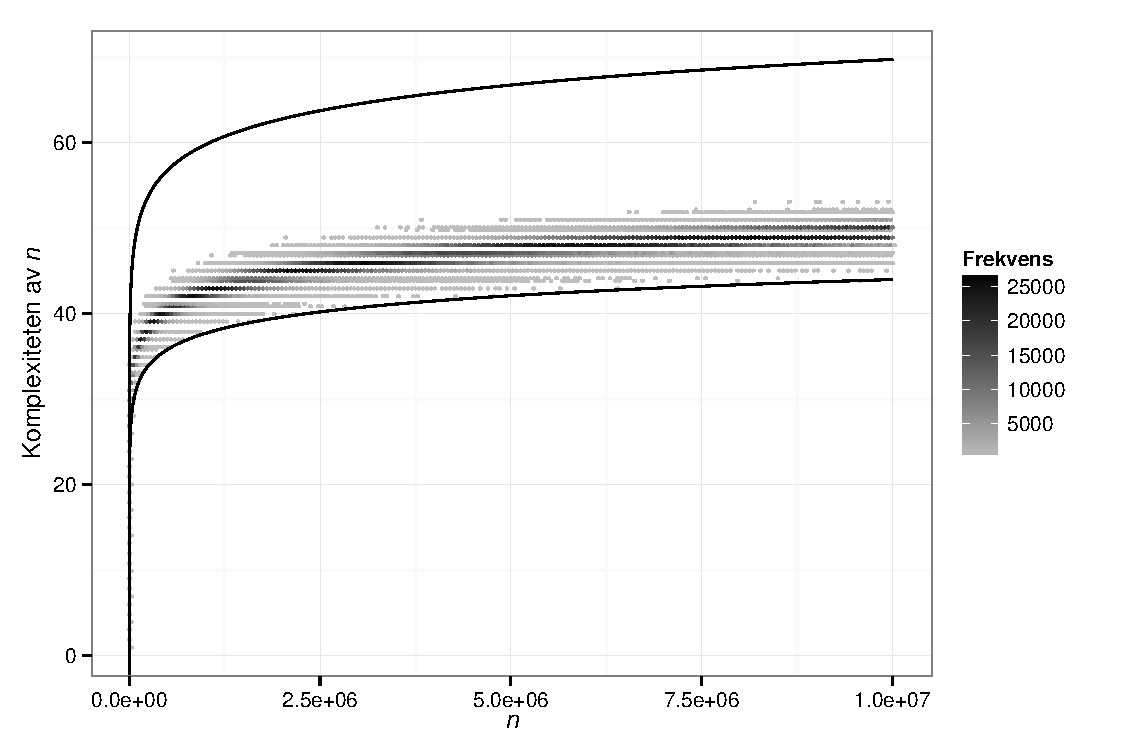
\includegraphics[width=\textwidth]{grafer/bounds}
        \caption{Graf över $\C{n}$ med den övre gränsen $3\log_2(n)$ och den undre $3\log_3(n)$}
        \label{bounds}
    \end{figure}

    Som man ser i \cref{bounds} är den undre gränsen så tight som det går, åtminstone som logaritmisk funktion. Den övre däremot ser ut att kunna
    förbättras en del, och där finns möjlighet för vidare forskning i framtiden.

    \begin{figure}[H]
        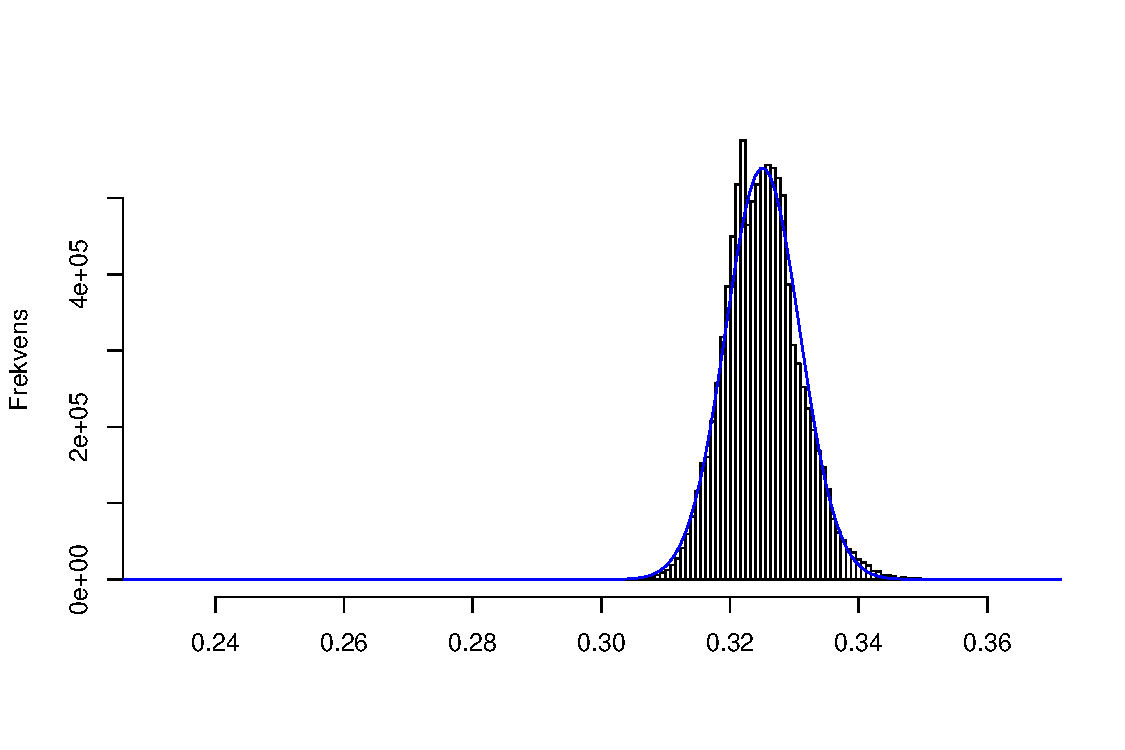
\includegraphics[width=\textwidth]{grafer/normhist}
        \caption{Histogram över $\frac{\ln(n)}{\C{n}}$ för alla $n\le10^7$ med anpassad normalfördelningskurva}
        \label{normhist}
    \end{figure}

    En annan intressant fråga är hur nära gränserna talen generellt sett ligger.
    Låt $ L(n) = \frac{\ln(n)}{\C{n}}$. Enligt \cref{undregrans} gäller

    $$3\log_3 n \le \C{n} $$
    $$\frac{\log_3 n}{\C{n}} \le \frac{1}{3}$$
    $$\frac{\ln n}{\C{n}} \le \frac{1}{3 \cdot \log_3(e)}$$
    $$ L(n) \le \frac{1}{3 \cdot \log_3(e)} \approx 0.366$$

    Den undre gränsen för $\C{n}$ ger alltså en övre gräns för värdet på $L(n)$, och desto närmre
    $\C{n}$ ligger den undre gränsen, desto närmre kommer $\L{n}$ ligga denna övre gräns.

    I \cref{normhist}

    \begin{figure}[H]
        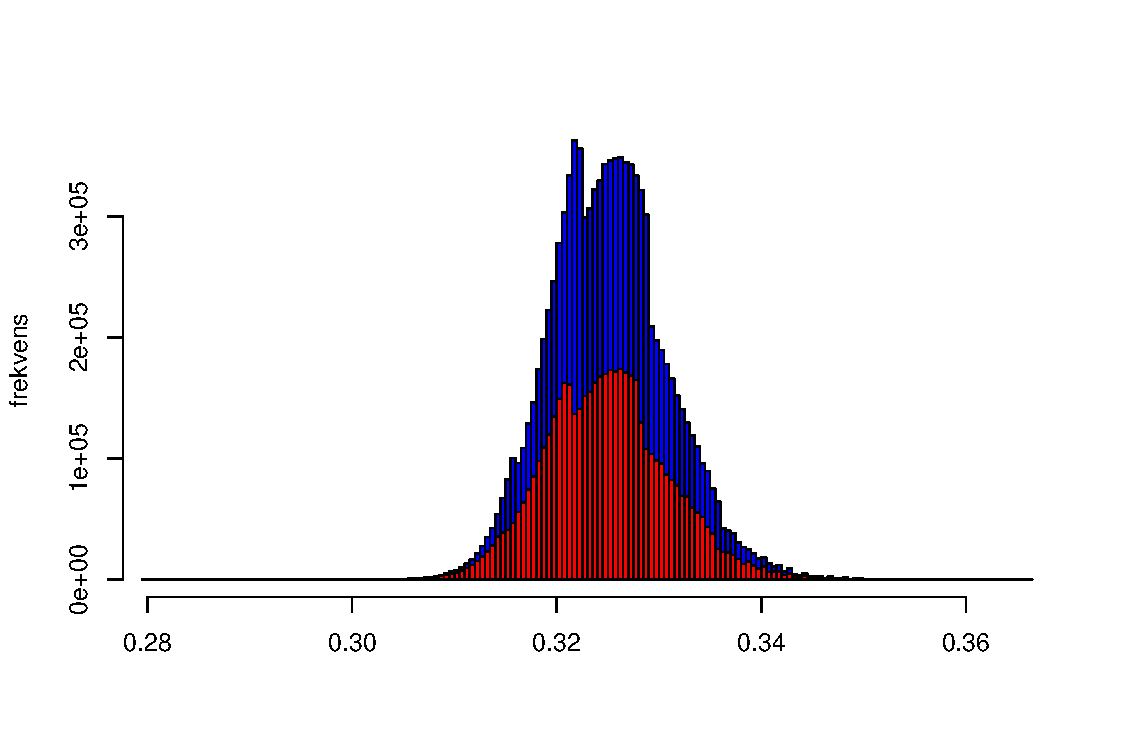
\includegraphics[width=\textwidth]{grafer/redblue}
        \caption{Histogram över $\frac{\ln(n)}{\C{n}}$. I blått $n\le10^7$ och rött $n\le5\protect\cdot10^6$}
        \label{redblue}
    \end{figure}

    \subsection{Speciella typer av tal}
    Då ingen explicit formel för $\C{n}$ har funnits, finns ett intresse i att undersöka huruvida
    samband existerar för specifika typer av tal. 
        \subsubsection{Kvadrattal}
        \begin{hypot}
            $\C{n^2}=2\cdot\C{n}$ \quad för alla $n\ge1$ \\
            Denna hypotes bevisas falsk genom motexemplet $n=5^4$ vilket ger $\C{n}=20$
            och $\C{n^2}=39<40=2\cdot\C{n}$.
        \end{hypot}

        \subsubsection{Primtal}
        \begin{hypot}
            $\C{p}=\C{p-1}+1$ \quad för alla primtal $p$ \\
            Detta är något som troddes vara sant väldigt länge, men som ingen
            lyckats bevisa. Med hjälp av de betydligt snabbare algoritmerna
            kunde man (VEM?) dock finna det minsta motexemplet $p = \num{353942783}$
            för vilket $\C{p} = 63 < 64 = \C{p-1}+1$.
        \end{hypot}

        \subsubsection{3-potenser}
        \begin{hypot}
            $\C{3^k}=3k$ \quad för alla $k\ge1$ \\
            Det är tydligt att $\C{3^k} \le 3k$ då:
            $$ 3^k = \underbrace{(1+1+1)(1+1+1)\ldots(1+1+1)}_{k \text{ st } (1+1+1) \text{ grupper}}$$
            Enligt \cref{undregrans} gäller:
            $$ \C{3^k} \ge 3\log_3(3^k) = 3k $$
            Alltså är $3k\le\C{3^k}\le3k$ så $\C{3^k}=3k$ och hypotesen är
            således bevisad.
        \end{hypot}
            



\section{Algoritmer för att generera sekvensen}

    För att generera data att undersöka söks en algoritm för att beräkna
    komplexiteten $\C{n}$ för ett tal.

    \subsection{En enkel algoritm}

    För att lösa frågan börjar vi baklänges, och ställer oss frågan: vilken ska den
    sista operationen vara?  Det är ju givet att representationen antingen kommer
    kunna sammanfattas som $n = a\cdot b$ eller $n = a+b$. Vi vill därför finna både rätt operation, och de två tal operationen ska
    utföras på. För att beräkna vilket som blir effektivast, behöver vi veta hur komplexiteten för alla de tal vi har som alternativ.
    Detta kan vi alltså lösa rekursivt och då vi kan anta att $a,b<n$ vet vi att
    algoritmen till slut kommer att komma till det basfallet $\C{1}=1$.
    Vi utnyttjar alltså:
    $$\C{n} = \min\Big[ \min_{1 \le k < n} \C{k}+\C{n-k}, \min_{k|n,1\le k}
    \C{k} + \C{\frac{n}{k}} \Big]$$

    En liten optimering är att för summan kommer vi behandla vissa fall dubbelt
    (både $k=t$ och $k=n-t$ ger samma resultat) så det räcker i algoritmen att
    endast behandla $k\le\floor{\frac{n}{2}}$. Liknande för multiplikationen
    ser vi att $k=t$ och $k=\frac{n}{t}$ ger samma resultat så det räcker att
    behandla $k\le\floor{\sqrt{n}}$.
        
    \begin{algorithm}[H]
        \caption{$\O(N^N)$}
        \label{nn}
        \begin{algorithmic}[1]
            \Procedure{complexity}{$n$}\Comment{Returnerar komplexiteten av n}
                \If{$n = 1$}
                    \LineComment{Vårt basfall, $\C{1} = 1$ ser till att algoritmen terminerar}
                    \State \Return $1$
                \EndIf
                \\
                \State  $ans\gets \infty$
                \\
                \LineComment{Kontrollerar alla möjliga summor av två tal}
                \For{$k\gets 1, \floor{n/2}$}
                    \State $ans\gets \min(ans, \textsc{complexity}(k)+\textsc{complexity}(n-k))$
                \EndFor
                \\
                \LineComment{Kontrollerar alla möjliga produkter av två tal}
                \For{$k\gets 2, \floor{\sqrt{n}}$}
                    \If{$k|n$}
                        \State $ans\gets \min(ans, \textsc{complexity}(k)+\textsc{complexity}(n/k))$
                    \EndIf
                \EndFor
                \\
                \State \Return $ans$
            \EndProcedure
        \end{algorithmic}
    \end{algorithm}

    Denna algoritm finner utan problem komplexiteten av tal upp till runt 20.
    Därefter blir den alltför långsam.

    En insikt kan dock förbättra vår metod och tillåta beräkning av komplexiteten
    för tal upp till 10 000 på under en sekund.

    Problemet innehåller nämligen många överlappande delproblem, och dessa löser
    algoritmen ett flertal gånger. Om vi istället sparar resultatet för varje tal
    kan de återanvändas, enligt en teknik som kallas dynamisk programmering. Vi
    sparar alltså $\C{n}$ i en lista $v[n]$ när vi har räknat ut komplexiteten
    av ett tal för att sedan återanvända resultatet om det skulle behövas.
    Vi låter för enkelhetens skull $v[n]=odefinerat$ från början. Förutom detta
    är algoritmen lika som den förra.

    Dessutom kan man göra algoritmen iterativ (d.v.s. att den inte är
    rekursiv) då det räcker att veta värdena på $v[k]$ för alla $k<n$ när
    man ska räkna ut $v[n]=\C{n}$. Vi fyller alltså upp listan $v$ i ordning.


    \begin{algorithm}[H]
        \caption{$\O(N^2)$}
        \begin{algorithmic}[1]
            \Procedure{complexity}{$maxN$}
                \\
                \LineComment{Basfallet}
                \State $v[1]\gets 1$
                \\
                \For{$n\gets 2, maxN$}
                    \LineComment{Här räknar vi ut $\C{n}$ på liknande sätt som
                    tidigare}
                    \State  $ans\gets \infty$
                    \For{$k\gets 1, \floor{n/2}$}
                        \State $ans\gets \min(ans, v[k]+ v[n-k])$
                    \EndFor
                    \For{$k\gets 2, \floor{\sqrt{n}}$}
                        \If{$k|n$}
                            \State $ans\gets \min(ans, v[k]+v[n/k])$
                        \EndIf
                    \EndFor
                    \State $v[n] \gets ans$
                \EndFor
                \\
                \LineComment{Nu är $v[n]=\C{n}$ för alla $n\le maxN$}
                \\    
            \EndProcedure
        \end{algorithmic}
    \end{algorithm}


    Att algoritmen nu är iterativ gör ingen skillnad i tidskomplexitet, men gör
    den i praktiken snabbare samt gör den något enklare att analysera.

    Denna procedur har en loop med två loopar inuti. Detta gör att en beräkning av
    $\C{n}$ tar proportionerligt mot $n\left(\frac{n}{2}+\sqrt n\right) =
    \frac{n^2}{2} + n\sqrt n$ tid.
    Eftersom vi räknar asymptotiskt spelar varken långsammare växande termer eller
    konstantfaktorer roll,  vilket innebär att algoritmen får tidskomplexiteten
    $\O(n^2)$.

    \subsection{En snabbare algoritm}
    Nedan följer en beskrivning av den förbättrade algoritm som beskrivs i \cite{algorithm_lune}.
    Den begränsande komplexiteten tidigare, var den hos loopen som kontrollerar den bästa möjliga summeringen. Denna gick från 1 till n/2. Vi söker nu ett nytt, mindre kMax, sådant att:
    $$\min\limits_{1 \leq k \leq n/2} \C{k} + \C{n-k} = \min\limits_{1 \leq k \leq kMax} \C{k} + \C{n-k}$$


    \subsubsection{Plan för algoritmen}
    Algoritmen kommer att bestå av av definition av hjälpfunktionen E, initiering av C[] samt en mainloop. När algoritmen terminerar kommer listan C[] ha fyllts av $\C{n}$ för
    $1 \leq n \leq nMax$. 

    \subsubsection{Hjälpfunktionen E}
    Först definieras en hjälpfunktion E enligt: för varje naturligt tal tal k, låt E(k) vara det största talet sådant att $\C{E(k)}$ = k.
    Notera att detta är samma funktion som definieras i \cref{undregrans}. Vi definierar ytterligare att $E(0) = 1$. Enligt formeln i \cref{undregrans} får vi följande algoritm för att beräkna E(k).

    \begin{algorithm}[H]
        \caption{$\O$}
        \begin{algorithmic}[1]
            \Procedure{E}{$n$}\Comment{Returnerar E(n)}
                \If{$n = 0$}
                    \State \textbf{return} $1$
                \EndIf
                \State $ans \gets 1$
                \While{n > 4}
                    \State $ans \gets ans \cdot 3$
                    \State $n \gets n-3$
                \EndWhile
            \State \textbf{return} ans
            \EndProcedure
        \end{algorithmic}
    \end{algorithm}



    \subsubsection{Funktionen kMax}
    Denna algoritm beräknar, med hjälp av E, tidigare nämna kMax för ett givet n. Notera att funktionen kräver att $\C{n}$ redan beräknats.

    \begin{algorithm}[H]
        \caption{$\O$}
        \begin{algorithmic}[1]
            \Procedure{kMax}{$n$}\Comment{Returnerar kMax(n)}
               \State $target \gets C[n-1] $
               \State $t \gets target/2 $
               \While{E(t)+E(target-1) < n}
                \State $t \gets t-1$
                \EndWhile
                \State \textbf{return} E(t)
            \EndProcedure
        \end{algorithmic}
    \end{algorithm}


    \subsubsection{Initiering av $C[\protect\cdot]$}
        Från början ska $C[\cdot]$ innehålla något tal som är större än den faktiska komplexiteten alla $1 \leq n \leq nMax$. Detta tal kallar vi $cMax$. Enligt
        \cref{ovregrans} så gäller att $\C{n} \leq  3\log_2 n$ \quad för alla $n\ge2$, så vi kan sätta $cMax =  \lf 3\log_2 n +1\rf$. Anledningen till att addera 1 är att eliminera risken för att de avrundningsfel som sker vid divisionen ska påverka resultatet.
        Vi sätter även $C[\cdot]=1$ eftersom detta är det kända värde som kommer användas för att få fram resten.
    \subsubsection{Mainloop}

        \begin{algorithm}[H]
        \caption{$\O(nMax^{1.230175})$}
        \begin{algorithmic}[1]
            \Procedure{Complexity}{$nMax$}
                \For{$n \gets 0, nMax$}
                    \If{$C[n-1]+1 < C[n]$} 
                        \State $C[n] \gets C[n-1]+1$
                    \EndIf

                    \For{$i \gets 6, kMax(n)$} \Comment Kollar summor
                        \State $sumans \gets C[i]+C[n-i]$
                        \If{$sumans < C[n]$}
                            \State $ C[n] \gets sumans$
                        \EndIf
                    \EndFor
                    \For{$i \gets 2, min(n, nMax/n)$}
                        \State $prodvalue \gets C[i]+C[n]$
                        \If {$prodvalue < C[i \cdot n]$}
                            \State $C[i \cdot n] \gets prodvalue$
                        \EndIf
                    \EndFor
                \EndFor
            \EndProcedure
        \end{algorithmic}
    \end{algorithm}

\subsubsection{Bevis}

\subsubsection{Tidskomplexitet}

\subsection{Fler algoritmer och diskussion}
 
Av de algoritmer som beskrivs, finns en stor variation i kvalitet och användbarhet. Den första är den enklaste möjliga algoritmen för
beräkning av $\C{n}$, men praktiskt relativt oanvändbar. Till $\O(n^2)$-algoritmen är steget inte långt, då dynamisk programmering får
anses vara en standardmetod, ändock är vinsten i tid enorm.
Den mest optimerade algoritm som finns för tillfället, är Fuller's algoritm, som även den beskrivs i \cite{algorithm_lune}.
Algoritmen har samma tidskomplexitet som algoritmen som beskrivs ovan, men bättre minneskomplexitet. Den är dock något mer komplicerad,
och beräknar endast svaret för ett enda tal, istället för alla tal upp till det. 
 \begin{tabular}[pos]{|l | c | c |}
 \hline
  \textbf{Algoritm} & \textbf{Tidskomplexitet} &  \textbf{Minneskomplexitet}\\ \hline
Rekursiv brute force & $\O(n^n)$ & b\\ \hline
Dynamisk programmering & $\O(n^2)$ & $n \cdot \log \log n$\\ \hline
Optimerad dynamisk programmering & $\O(n^{1.230175})$ & 0.6584 \\ \hline
Fuller's algoritm & $\O(n^{1.230175})$ & 0.7159\\ \hline

\end{tabular} \\

\newpage
\begin{thebibliography}{9}

    \bibitem{spansk}
        \text{J. Arias de Reyna}, \emph{Complejidad de los n'umeros naturales}, 2000
     \bibitem{algorithm_lune}
     	\text{J. Arias de Reyna, J. Van de Lune}, \emph{Algorithms for Determining Integer Complexity}, arXiv: 1404.2183v2

\end{thebibliography}
%\bibliography{bib}{}
%\bibliographystyle{unsrtnat}

\end{document}

